%
% File acl2019.tex
%
%% Based on the style files for ACL 2018, NAACL 2018/19, which were
%% Based on the style files for ACL-2015, with some improvements
%%  taken from the NAACL-2016 style
%% Based on the style files for ACL-2014, which were, in turn,
%% based on ACL-2013, ACL-2012, ACL-2011, ACL-2010, ACL-IJCNLP-2009,
%% EACL-2009, IJCNLP-2008...
%% Based on the style files for EACL 2006 by 
%%e.agirre@ehu.es or Sergi.Balari@uab.es
%% and that of ACL 08 by Joakim Nivre and Noah Smith

\documentclass[11pt,a4paper]{article}
\usepackage[hyperref]{acl2019}
\usepackage{times}
\usepackage{latexsym}
\usepackage{graphicx}
\usepackage{amsmath}
\usepackage{amssymb}
\usepackage{booktabs}
\usepackage{url}

\usepackage{color}
%\aclfinalcopy % Uncomment this line for the final submission
%\def\aclpaperid{***} %  Enter the acl Paper ID here

%\setlength\titlebox{5cm}
% You can expand the titlebox if you need extra space
% to show all the authors. Please do not make the titlebox
% smaller than 5cm (the original size); we will check this
% in the camera-ready version and ask you to change it back.

\newcommand\BibTeX{B\textsc{ib}\TeX}

\DeclareMathOperator{\softmax}{softmax}
\DeclareMathOperator{\sigmoid}{sigmoid}

\definecolor{Orange}{RGB}{255,140,0}
\definecolor{Blue}{RGB}{0,191,255}
\newcommand{\ek}[1]{\textcolor{Orange}{[ek: #1]}} 
\newcommand{\cp}[1]{\textcolor{Blue}{[cp: #1]}}

\newcommand{\word}[1]{\emph{#1}}

\newcommand{\aout}{\mathbf{a_{\text{out}}}}


\definecolor{Red}{RGB}{255,0,0}
\newcommand{\red}[1]{\textcolor{Red}{#1}}
\newcommand{\jd}[1]{\textcolor{Red}{[jd: #1]}} 

% \title{Predicting guilt judgments from crime stories}
\title{Attention Weights as a Window into How Crime Narratives Shape Subjective Assessments of Guilt}

\author{Elisa Kreiss \\
  Department of Linguistics \\
  Stanford University \\
  \texttt{ekreiss@stanford.edu} \\\And
  Judith Degen \\
  Department of Linguistics \\
  Stanford University \\
  \texttt{jdegen@stanford.edu} \\\And
  Christopher Potts \\
  Department of Linguistics \\
  Stanford University \\
  \texttt{cpotts@stanford.edu}\\}

\date{}

\begin{document}
\maketitle
\begin{abstract}
  Neural network attention mechanisms have led to performance gains on a wide variety of tasks in natural language understanding, and they have also provided clues as to how these complex networks represent the language they process, opening up new avenues for linguistic investigation. In this spirit, we apply neural networks with attention to the task of modeling human judgments about guilt based on short crime narratives. The networks are successful at the task, and probing their attention weights helps illuminate the ways in which they make use of markers of certainty and uncertainty in different crime narratives. The findings reflect the pragmatic complexity of these linguistic devices, and they suggest new ideas about how crimes might be more effectively reported in the news media.
\end{abstract}

\section{Introduction}

Deep learning models are increasingly applied to language tasks not just to develop technologies but also to derive new insights into language use. These more scientific applications raise the question of whether these models process data in a motivated way; their ``black box'' nature is often an obstacle to answering this question \citep{Alishah-etal:2019}. Recently, attention mechanisms, which capture the strength of association between components of these networks \citep{bahdanau2014neural,luong-etal-2015-effective}, have not only improved performance, but also increased interpretability, potentially opening the door to new linguistic applications of these models (but see \citealt{Serrano:2019} for a critical perspective).

In this paper, we apply neural networks with attention to a task that has both linguistic and societal import: predicting whether the reader of a short narrative crime report will conclude that the main subject is guilty or innocent. Our networks rely on the attention mechanisms of \citet{Lin:2017}, which learn a weighting of the words in examples based on their contribution to the output prediction. These networks achieve strong performance on the task, as defined by the dataset of \citet{Kreiss:2019}, which leads us to explore their learned parameters by inspecting how they make predictions for new, carefully controlled inputs.

We find that the networks make robust use of markers of certainty and uncertainty, as well as discourse connectives that signal contrast. In addition, by systematically removing this language from test examples, we find that these markers have a large impact where the evidence is weak but have little or no impact where the evidence is strong. These findings align well with the well-known semantic and pragmatic complexity of hedges and other epistemic markers \citep{Simons07,vonFintel:Gillies:2010,deMarneffe:Manning:Potts:2012,White-etal:2018}. In addition, to the extent that humans adopt similar reading strategies, this can inform how the news is reported, in that it yields insights into the complex ways that words like \word{allegedly} and \word{possibly} shape readers' construals of newspaper articles \citep{Erickson-etal:1978,jensen2008scientific}.


\section{Related Work}

Our work draws on prior research concerning the relationship between language and assessments of guilt, as well as work seeking to use neural networks to inform linguistic theory.


\subsection{Predicting Guilt}
% 1. Topic sentence (e.g., "There is extensive prior literature on how linguistic markers influence perceptions of guilt").
The challenge of predicting guilt judgments from text sources has not yet received much attention. 
% 2. Basically a list of papers falling under the topic, with basic details about what the work does.
However, \citet{Fausey:Boroditsky:2010} show that using agentive language increases blame and financial liability judgments people make. Their results suggest that even subtle linguistic changes in crime reports can shape people's judgments of the events.
More recent work has focused on predicting guilt verdicts from the Supreme Courts in the Philippines \citep{virtucio2018predicting} and Thailand \citep{kowsrihawat2018predicting} on the basis of presented facts  and legal texts. \citeauthor{kowsrihawat2018predicting} employ a recurrent neural network with attention to make these predictions.
% 3. A final section explaining how the above relates to the current paper.
This previous work is not concerned with the linguistic basis of subjective guilt judgments, but rather with courtroom verdicts based on legal texts. Here we instead focus on subjective guilt judgments, and we train networks not primarily for their predictive capacity, but rather to probe their learned parameters.


\subsection{The Interpretation of Hedges}

% 1. Topic sentence (e.g., "There is extensive prior literature on how linguistic markers influence perceptions of guilt").
Researchers have categorized (un)certainty markers in numerous ways (e.g., \citealt{lakoff1972hedges, prince1982hedging, brown1987politeness}). For a summary, we refer readers to \citealt{fraser2010pragmatic}. 
In this work, we use ``hedge'' broadly, as an umbrella term for all subclasses of uncertainty markers, including any marker that, as \citet{prince1982hedging} says, introduces uncertainty ``within the propositional content'' (e.g., \word{His feet were \textbf{sort of} blue}) or ``in the relationship between the propositional content and the speaker'' (e.g., \word{\textbf{I think} his feet were blue}).

% 1. Topic sentence
There is extensive prior literature on how hedges affect perceptions of the speaker and proposition \citep{Erickson-etal:1978, durik2008effects, bonnefon2006tactful, rubin:2007:ShortPapers, jensen2008scientific, ferson2015natural}.
% 2. Basically a list of papers falling under the topic, with basic details about what the work does.
These studies suggest that hedges affect people's judgments of credibility in differing ways. For example, an increase in the number of hedges decreases the credibility of witness reports \citep{Erickson-etal:1978}, but, at the same time, increases the trustworthiness of journalists and scientists \citep{jensen2008scientific}. Additionally, the interpretation of hedges is context dependent \citep{bonnefon2006tactful,durik2008effects,ferson2015natural} and shows high individual variation \citep{rubin:2007:ShortPapers,ferson2015natural}. 
% 3. A final section explaining how the above relates to the current paper.
Since neural networks can be trained flexibly in many different environments, they hold the promise of systematically studying this kind of variation at scale -- as long as their representations are interpretable.

In addition, computational and theoretical work on veridicality has revealed that not all hedges serve merely to reduce speaker commitment. For instance, attitude predications like \word{The company reported S} and \word{They said S} are often used to convey evidence sources. In such utterances, the speaker might wish to appear fully committed to the embedded content \word{S} despite the apparent hedging \citep{Simons07,deMarneffe:Manning:Potts:2012,White:Rawlins:2018,White-etal:2018}. Similarly, \citet{vonFintel:Gillies:2010} show that related evidential readings arise for epistemic \word{must}. These findings show how complex these markers are pragmatically and highlight the value of usage-based studies of them.


\subsection{Linguistic Insights from Neural Networks}

Neural networks were originally motivated largely by questions in cognitive science \citep{pater2019generative}, especially concerning issues of representation and learning (e.g., \citealt{rumelhart1986learning,tesar2000learnability}). Today, they are more closely associated with engineering efforts, but there is increasing interest in returning to these models' cognitive motivations and in using them to try to gain insights about linguistic phenomena.

An obstacle to this work is the incredible representational power of these networks, which can make their representations inscrutable. However, recent efforts are overcoming this. For instance, \citet{N16-3020} and \citet{Koh:Liang:2017} develop general methods for probing complex models to understand which features  guide their predictions. Attention weights are increasingly playing a role in such efforts. For instance, \citet{jawahar-etal-2019-bert}, \citet{clark2019what}, and \citet{tenney-etal-2019-bert} present evidence that BERT language models systematically encode core aspects of linguistic structure. We present a similar argument here, but focused on usage-based patterns.\jd{not sure i understand what this last sentence is supposed to mean}

Finally, \citet{linzen-etal-2016-assessing} argue for applying methods from psycholinguistics to trained neural networks, treating them as participants whose behavior we can observe and learn from (see also \citealt{gulordava-etal-2018-colorless,Futrell-etal:2019}). We employ similar methods to home in on which words our models are most attuned to.


\section{Dataset}\label{sec:dataset}

\begin{table*}
\centering
\begin{tabular}{p{.45\textwidth} p{.45\textwidth}}
  \toprule
  \multicolumn{2}{p{0.925\textwidth}}{On August 30 2018, 30,000 internet users in Spain received an email with the subject line `Immediate response required -- copyright infringement'. In these emails, the recipients were accused of illegally distributing pornographic content and were instructed to pay \$11,500 by the end of September to avoid a lawsuit. Searching for the email address online leads to an official law firm website located in Barcelona. Shortly after the emails were sent out, the law firm disowned them, calling them a hoax. So far, police officials estimate that approximately 5\% of the recipients have paid the money. This sums to more than \$17 million that have been paid to the scammers. Now, nearly 4 weeks later, the police have tracked down the internet cafe from which the emails were sent. After observing the cafe's camera footage, the police arrested a man and a woman (both 52) who were allegedly responsible for the scam. If found guilty, they face up to 9 years in prison.}\\ 
  \midrule
  (\emph{strong evidence condition}) & (\emph{weak evidence condition})  \\
  Moreover, news outlets recently acquired access to the camera footage and found that the video material is of very high quality and therefore undoubtedly reliable. & However, news outlets recently acquired access to the camera footage and found that the video material is of very poor quality and therefore potentially unreliable. \\ 
  \bottomrule
\end{tabular}
\caption{Example of a seed story in the two conditions from the Annotated Iterated Narration Corpus (AINC).}
\label{tab:examplestory}
\end{table*}

Our experiments rely on the Annotated Iterated Narration Corpus (AINC) collected by \citet{Kreiss:2019}.\footnote{\url{https://github.com/elisakreiss/iterated_narration}\ek{TODO: add proper corpus link!}} The corpus was created for investigations into how news stories change when they are propagated from one person to another.

First, the authors created five stories of approximately 850 words, which are called the \emph{seed} stories. All of them report a crime and an arrest of one or more suspects. Each of these five seed stories exists in a weak and a strong evidence condition. The stories are identical up to the last phrase, which then either raises doubts about the arrest or emphasizes its validity. For example, if a suspect was arrested on the basis of camera footage, this footage was described as being of ``very poor quality'' in the weak evidence condition and ``very high quality'' in the strong evidence condition. Table~\ref{tab:examplestory} provides a complete example.

Each story was given to a participant who was asked to read and afterwards reproduce it. The reproduced story was then given to the next participant, who again reproduced it. The data collection therefore followed the transmission-chain paradigm introduced by \citet{Bartlett:1932}. Following this schema, each story and condition was reproduced in 5 chains over 5 generations, resulting in 250 reproductions and thus 260 stories overall.

\begin{figure}[tp]
  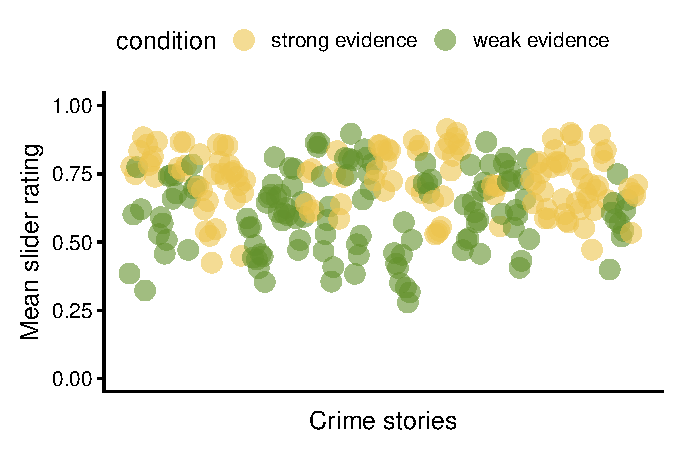
\includegraphics[width=\linewidth]{graphs/subjguilt.pdf}
  \caption{A point represents the mean subject guilt rating for a story in the corpus,
    color-coded for condition.\jd{why is this a scatterplot instead of a histogram or density plot?}}
  \label{fig:corpus-annotations}
\end{figure}

After the corpus collection, \citeauthor{Kreiss:2019}\ obtained human responses pertaining to a range of issues. Participants were recruited on Amazon Mechanical Turk. The questions were primarily related to different aspects of guilt perception but also, for example, perceived subjectivity of the story writing. We focus here on the question ``How likely is it that the suspect(s) in the crime is/are are guilty?'' Participants indicated their responses on a continuous slider labeled `very unlikely' at its lowest point and `very likely' at its highest. Each story received approximately 20 ratings. For the purpose of this work, we rescale the responses into $[0,1]$ and consider the mean rating for each story as its guilt judgment label. The labels of each story are shown in Figure~\ref{fig:corpus-annotations}. In contrast to the raw ratings, the means range only from $0.27$ to $0.92$. 

In summary, the AINC is a corpus of reproduced news stories, annotated with human guilt judgments. Since the stories originated from only 5 unique stories (each in 2 conditions), a lot of information is shared between single data points.  Despite this similarity, the range of guilt judgments is still high, alluding to subtle differences that trigger this variance. We now turn to the question of whether a deep learning model can learn to predict the assessments of guilt the corpus provides.


\section{Model}\label{model-architecture}

\begin{figure}[tp]
  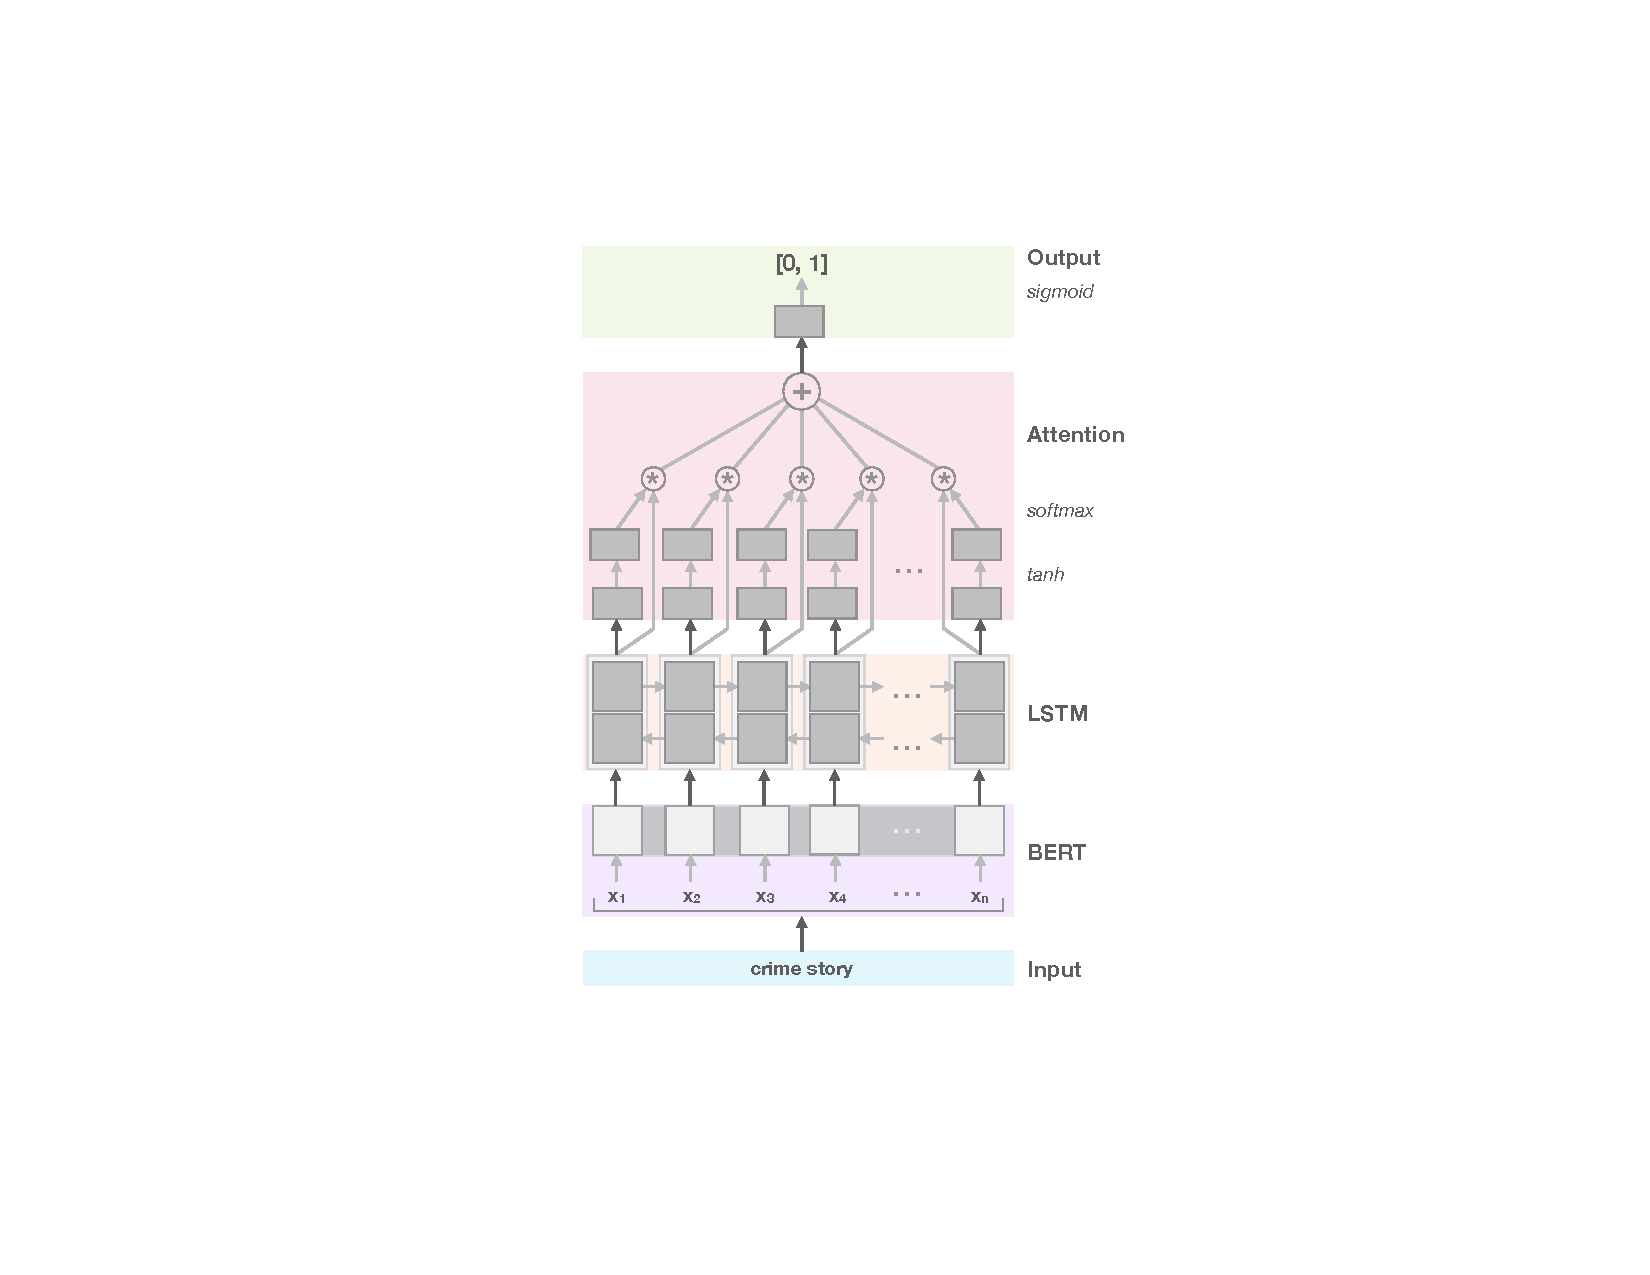
\includegraphics[width=1\linewidth]{graphs/model.pdf}
  \caption{Model architecture. The BERT layer produces
    a sequence of context-dependent representations. These
    are the inputs to the bidirectional LSTM, which
    fine-tunes these representations to our task.
    The LSTM outputs feed into the attention layer,
    which produces a summary representation of the full
    text that is weighted by each word's contribution
    to the final predictions.}
  \label{fig:model}
\end{figure}

Our model is based on that of \citet{Lin:2017}, which is fundamentally a  bidirectional LSTM with attention mechanisms applied to its outputs. We chose this model primarily because its attention mechanisms seem especially promising for introspection, as they essentially provide a weight for each word in the input, and this weight controls how much each word contributes to the network's final predictions. The overall architecture is summarized in Figure~\ref{fig:model}.

% The goal of this work was to determine whether neural networks can be a useful tool to investigate the formation of guilt judgments. To do this, we used a model which was based on the design proposed by \citeauthor{Lin:2017}. We chose to use this model as our base because of its promising performances in various NLP tasks. Furthermore, its attention module provides a straightforward way to investigate the inner workings of the model.


The only major adjustment we made to the model is that we replaced the GloVe word embeddings \citep{Pennington:2014} by BERT representations \citep{Devlin:2018}. Whereas GloVe provides a single embedding for each word, with no sensitivity to the context in which it occurs, BERT representations vary by syntactic context. \citeauthor{Devlin:2018}\ report that using these embeddings boosts performance in all of the natural language tasks they consider, and we saw comparable improvements when we switched from GloVe to BERT. To access pretrained BERT parameters, we used the Hugging Face toolkit.\footnote{\url{https://github.com/huggingface/pytorch-transformers}}

We allow BERT to tokenize the input string according to its internal tokenization method \citep{wu2016google}, to make maximal use of its own pretrained embedding. These token representations are processed by BERT using its pretrained Transformer parameters \citep{Vaswani:2017}, yielding a sequence of contextual representations for them. These are fed into a bidirectional LSTM layer in which each cell's output has dimension $200$. The two representations at each step are concatenated to form the LSTM layer output for each token.

For the attention layer, we follow the design of \citeauthor{Lin:2017}: the LSTM outputs are organized into a matrix $H$ of dimension $n \times 400$, where $n$ is the token length of the current sequence, and we apply a dense layer with parameters $W$ (dimension $50 \times 400$) and a $\tanh$ activation to create a matrix $A$ of $50$-dimensional representations for each token:
%
\begin{equation}
  A = \tanh(WH^{\top}) \label{eq:A}
\end{equation}
%
Using learned weights $\mathbf{w}$ (dimension $1 \times 50$), the matrix $A$ is further compressed to the attention weight vector $\mathbf{a}$ of size $1 \times n$, with a softmax applied so that the weights sum to $1$:
%
\begin{equation}
  \mathbf{a} = \softmax(\mathbf{w} A) \label{eq:attn}
\end{equation}
%
\citeauthor{Lin:2017} actually generalize this attention operation to return a matrix with $r$ attention weights for each token. We set $r=1$ to keep the number of parameters low and increase the interpretability of the network.

Finally, we take the dot product of the LSTM hidden state matrix $H$ and the just obtained vector $\mathbf{a}$ to obtain the attention layer output vector $\aout$ of size $1 \times 400$:
%
\begin{equation}
  \aout = \mathbf{a}H \label{eq:aout}
\end{equation}
%
This is a compressed representation of the entire input sequence. Intuitively, the attention weights capture the relative importance of each token with regard to the final prediction, and $\aout$ synthesizes all of these weighted contributions into a single vector.

Finally, the logistic regression module makes a guilt prediction. For this step, $\aout$ is linearly transformed into a single number $p = \sigmoid(\mathbf{x}\,\aout^{\top} + b)$, where $\mathbf{x}$ is a vector of regression weights (dimension $1 \times 400$) and $b$ is a bias term. The sigmoid function ensures that the prediction lies between $0$ and $1$, just like the restriction on the guilt judgments it is trained on.

Overall, the model has $111,054,742$ trainable parameters. This sounds mismatched with our very small dataset, but only $0.02\%$ of these parameters are in the attention and output modules and $1.40\%$ are in the LSTM module. The rest of the parameters ($98.59\%$) are the pretrained weights in the BERT word embedding module, so they actually help us get traction on our small dataset by bringing in a lot of outside linguistic knowledge.


\section{Experiment}

Our initial goal is to assess the extent to which our bidirectional LSTM with self-attention (as described in Section~\ref{model-architecture}) can predict human guilt judgments from news stories. Assuming the model succeeds, we can then probe its internal representations for linguistic insights.

\begin{figure*}
  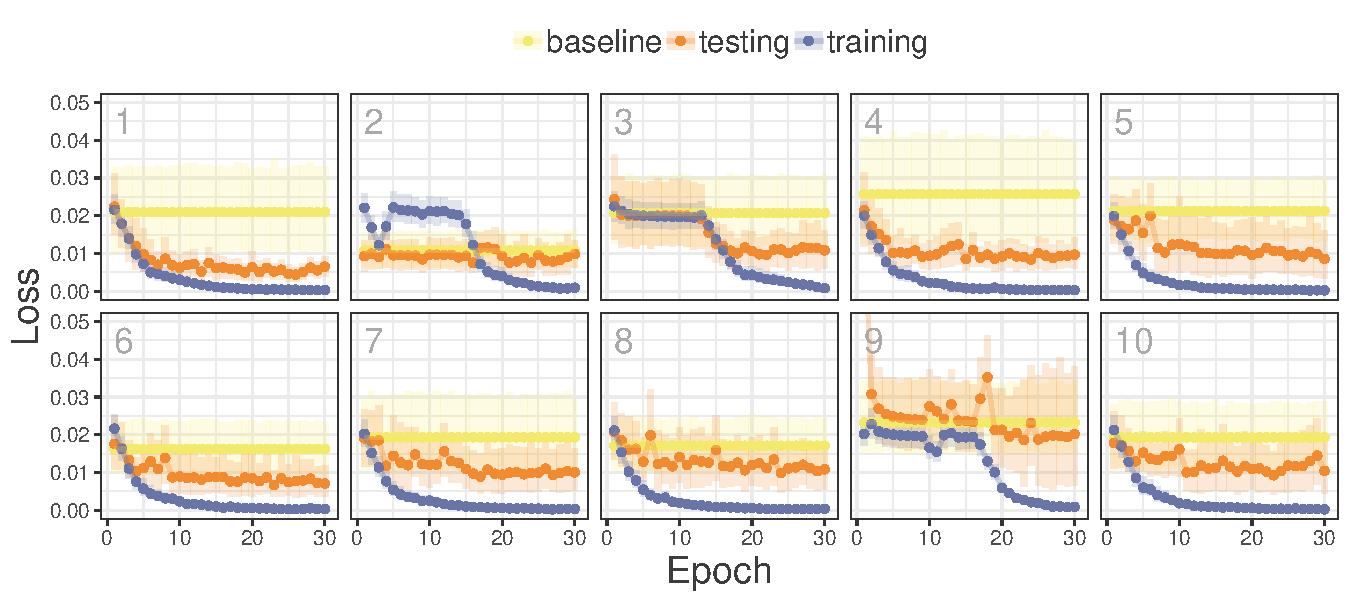
\includegraphics[width=\linewidth]{graphs/lossPlotCropped.pdf}
  \caption{Loss (mean squared error) over epochs (x axis), faceted over cross-validation configurations. The performance of the model on the training set (in blue) approaches zero. The performance of the model on the dev-test set (in orange) generally outperforms the baseline (in yellow).}
  \label{fig:loss}
\end{figure*}

\subsection{Optimization}

To begin, we held out 26 randomly selected stories (from the 260 stories in total) as the final test set. The remaining 234 stories were then used for model training and validation, which was done using 10-fold cross validation. The cross-validation results inform us about the model variation observed across train/validation splits. It is likely that, given the small size of the dataset, this variation will be high, so we want to be attuned to it.

In each step of the 10-fold cross-validation, the model was trained on 206/207 stories and 23/24 were held out for dev-testing. As noted above, the predicted guilt rating was the mean participant guilt rating obtained from the previously described data collection and annotation.

For training, the model uses mean squared error (MSE) as the loss function, stochastic gradient descent as the optimizer, and a learning rate of $0.1$. The model was implemented using PyTorch \citep{Paszke:2017}. It was trained for 30 epochs, for each of the 10 train/dev-test configurations in the cross-validation.


\subsection{Results}

Figure~\ref{fig:loss} shows the MSE loss for each training epoch. We show the dev-set loss for our model (orange) as well as the train-set loss (blue). In addition, to provide context for the results, we include the loss for a dummy regressor that predicts the mean of the training data labels for all cases.

The training loss approaches $0$ toward the end of the training in all cross-validation configurations, indicating model convergence. Crucially, our model's dev-set performance is always substantially better than the baseline model, indicating that the model is indeed learning from the dataset. That said, there is a high amount of variation between the different cross-validation steps, with the baseline actually proving competitive in some folds. This seems an inevitable consequence of our small dataset, but the model clearly has gotten traction on the problem overall.

% The mean of the training labels alone (i.e., the baseline) only has a very small loss on cross-validation configuration 2 and the trained model can barely beat it. This is in clear contrast to cross-validation step 4, where the baseline model loss is very high on the dev-test data and the trained model can easily surpass it. Those two cases exemplify the high variation that comes with the different splits of training and dev-testing data\footnote{However, I cannot exclude that also the random parameter initialization plays a relevant role here. But at least the differences in the baseline are definitely caused by the different splits.}.

The MSE loss alone is not sufficient to assess how well the model actually learns to predict the underlying distribution. Figure~\ref{fig:corr-cv0} shows the correlation between the actual target labels (on the x axis) and the model predictions (on the y axis) for one of the cross-validation folds. Before training (left), the models are undifferentiated. After training (right), the model predictions (blue) are highly correlated with the true labels ($r=0.85$), and the MSE is small ($0.007$).

Qualitatively, these plots appear very similar throughout all cross-validation configurations and can be compared in Figure~\ref{fig:app-corr-pretraining} and \ref{fig:app-corr-posttraining} in the Appendix. Quantitatively, the correlation on the dev-test set does show variation, driven mainly by outliers.
% That's plausible but I don't know that for these outliers
% \footnote{In particular, the story about sexual harassment allegations against a male professor proved to look different from all the rest. It's the only story with a clear and relevant gender difference between victim(s) and suspect. \citet{Erickson-etal:1978} show that powerless style (which includes hedges) affects credibility ratings dependent on power structures.\label{fn:prof}} 
However, overall, the mean correlation between the model prediction and the human judgment on the testing set across all cross-validation steps is $0.68$. When we collapse over all cross-validation folds and examine the loss after training, the difference in loss between the model predictions and baseline is significant ($p<0.0001$) according to a linear regression.

As a final performance evaluation, we examine the target--prediction correlation on the held-out test set (Figure~\ref{fig:test-corr}). For predictions on the test set, we used the final model weights obtained by the first cross-validation configuration. This fold's model was chosen because of its low dev-set loss and strong predictions. This was the only evaluation that was performed on this held-out test set. The Pearson correlation on the held-out test set is still high ($0.84$) and almost identical with performance on the dev-set for this fold. This high correlation, and the fact that the high correlation reproduces with the held-out testing data, indicates that the model was able to learn to generalize accurately to new cases in our domain.

\begin{figure}
  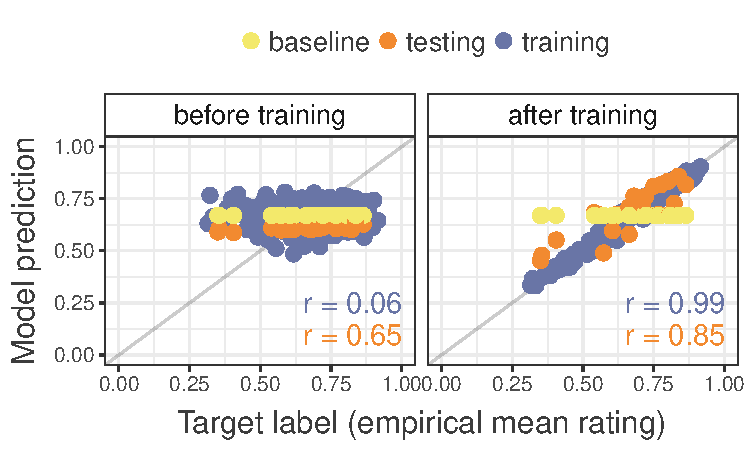
\includegraphics[width=\linewidth]{graphs/cv0-pred-target-epoch0-29.pdf}
  \caption{Correlation between target label (x axis) vs.\ model prediction (y axis) before and after training.}
  \label{fig:corr-cv0}
\end{figure}

\begin{figure}
  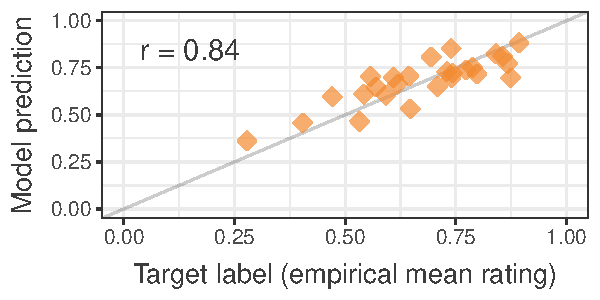
\includegraphics[width=\linewidth]{graphs/test-corr.pdf}
  \caption{Testing label (x axis) vs.\ model prediction (y axis) after training on the held out test set (26 data points) using the parameter settings obtained after the 30th epoch from the first cross-validation. The Pearson correlation is $0.84$.}
  \label{fig:test-corr}
\end{figure}


\section{Model analysis}

We have established that the proposed model can predict human guilt judgments when given a crime story. This result invites us to ask whether there are patterns underlying these predictions that can provide higher-level insights into how language is construed in these criminal contexts. 

\begin{figure*}[t]
  \centering
  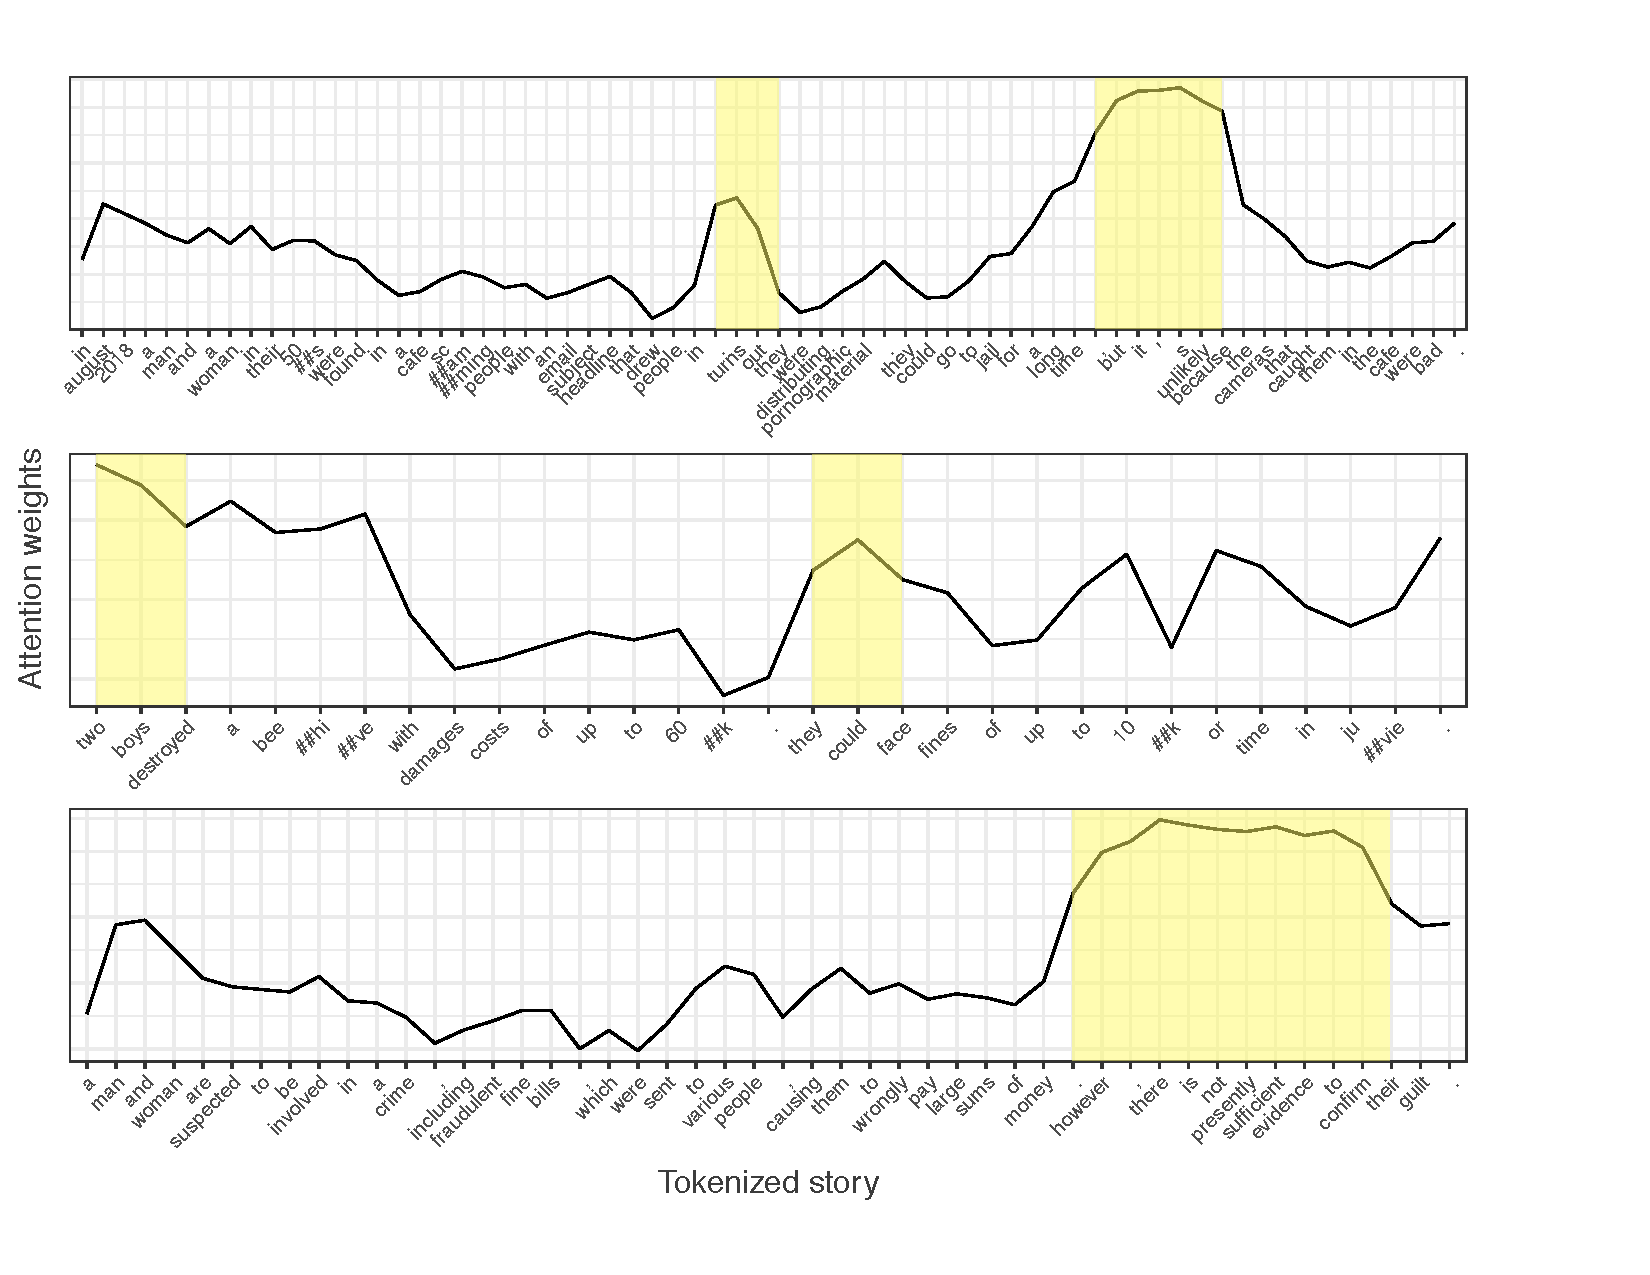
\includegraphics[width=1\linewidth]{graphs/attention-marked.pdf}
  \caption{Visualization of the attention weights (y axis) for a tokenized story (x axis) from the test set. Because we took the softmax over the attention weights, the scale of the y axis is irrelevant. Areas of high attention weight are marked in yellow and correlate with markers of (un)certainty as well as markers of contrast.\jd{A, B, and C come from different stories, no? indicate in caption?}}
  \label{fig:viz}
\end{figure*}

\subsection{Visualization}

We begin by inspecting the learned attention weight vector $\mathbf{a}$ in equation (\ref{eq:attn}). Since the softmax forces the sum of the weights to be 1, we cannot interpret the weights on their own for each word or across stories. Instead, the relevance lies in the differences between words and phrases within each story, and patterns of similarities between stories.

To investigate what might affect model predictions, we ran the model again on the final test data. Figure~\ref{fig:viz} displays three of these stories with their attention weight distribution.
We see that the model seems to focus on phrases that explicitly describe uncertainty about the evidence (see Figure~\ref{fig:viz}C). If present, these cues usually outweigh the rest of the story. This suggests that, if there is an explicit claim that affects the evidence of the suspect's guilt, it is considered as the most important source to inform guilt judgment.

Additionally, peaks occur on words and phrases which convey contrast, such as \word{however}, \word{but}, \word{even though}, and \word{it turns out}. This can be seen in all three stories in Figure~\ref{fig:viz}. These phrases not only correspond to turning points in the story, but also tend to signal argument structure, changes in expectations, and concessions \citep{RLakoff:1971,Merin:1999,Blakemore01}. In our stories, these markers mostly follow reports of arrests, so they might be correlated with objections to those arrests which would influence guilt perceptions.

Figure~\ref{fig:viz}B shows a case where the model seems to find a simple declarative (\word{two boys destroyed}) to be relevant for the final prediction. This is especially interesting because declaratives on their own do not generally communicate guilt-related information. However, they are very important for guilt judgments because they do not allow any uncertainty about the association between crime and suspect.

In summary, visualizing the attention weights contributes further evidence that the model has learned meaningful patterns in the data, and suggests that we can use the network to understand the role of specific words and phrases in shaping guilt judgments.


\subsection{Qualitative Analysis}

Figure~\ref{fig:viz} provides evidence for the claim that the model picks up on meaningful patterns in the corpus. \jd{for three cherry-picked examples, yes. is there any way to quantify this? eg, you've annotated all the hedges. could one do sth simple like test the extent to which, within one sentence, mean attention to hedges is greater than to other expressions?} But does the model make reasonable predictions on newly constructed examples?  The original corpus started out with 5 different crime stories. Each of these stories occurred in 2 conditions -- one suggesting that the evidence that led to the arrest was weak, and the other that the evidence provided a strong case. Additionally, the stories were filled with uncertainty markers such as \word{allegedly} and \word{(un)likely}, which we expect to have an impact on guilt judgments. However, the corpus cannot inform us about this relationship.

\begin{figure}
  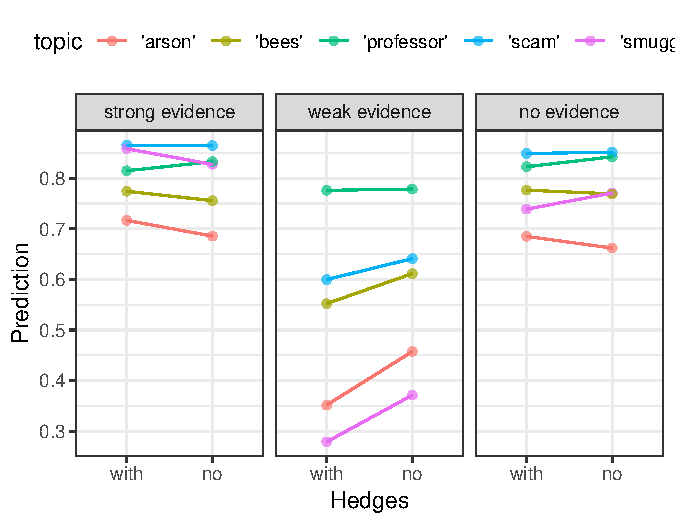
\includegraphics[width=1\linewidth]{graphs/hedges.pdf}
  \caption{Model predictions for our hedge manipulation. In the `with' condition,
    the original hedges are left in the stories; in the `no' condition, they are
    carefully edited out. In the strong evidence condition, this has no discernible
    effect. However, in the weak evidence condition, removing these markers
    consistently increases guilt judgments. 
    The only exception is the outlier `professor' story mentioned in footnote~\ref{fn:prof}. 
    In the `no evidence' condition, the evidence statement is simply removed.}
  \label{fig:hedges}
\end{figure}


We can, though, use the model to predict a guilt judgment for each of the original stories without these uncertainty markers/hedges. Thus, we rewrote those 10 original stories into versions without any uncertainty markers. They remained as close to the original as possible, while still remaining grammatical. Figure~\ref{fig:hedges} summarizes this analysis.

The results suggest that uncertainty markers have different effects on guilt prediction in the two evidence conditions. When the evidence is strong (right panel), removing the uncertainty markers does not affect guilt judgments. However, when the evidence is weak (middle panel), removing those hedges increases guilt judgments.\footnote{The only exception is the outlier `professor' story, which is a story about sexual harassment allegations against a male professor. It's the only story with a clear and relevant gender difference between victim(s) and suspect. \citet{Erickson-etal:1978} show that powerless style (which includes hedges) affects credibility ratings dependent on power structures.\label{fn:prof}} This has an intuitive interpretation: when the evidence already overwhelmingly speaks for the suspect's guilt, it outweighs the hedges; when the evidence is questionable, other sources of uncertainty are considered to inform a final judgment.

Finally, we can remove the evidence statement entirely and see how the network responds (right panel). What we find is that the predictions fall into the same overall range as for the strong evidence condition, regardless of whether the hedges are included or not. This suggests that our model is defaulting to a presumption of guilt, and that hedges alone do not suffice to alter that bias -- explicitly weak evidence is required for that.


\section{Discussion}

We applied a neural network with attention mechanisms to the task of predicting subjective guilt judgments in the Annotated Iterated Narration Corpus of \citet{Kreiss:2019}. Though this corpus is small, our network was able to learn effectively from it, which opened the door to studying its learned parameters to see whether they can yield linguistic insights. In visualizing the attention weights, we observed that the network attends closely to markers of (un)certainty and contrast, which aligns with pragmatic characterizations of this language. However, in systematically varying examples to remove the (un)certainty markers, we uncovered an additional dimension to this finding: only where the evidence given is explicitly weak do these markers play a large role in shaping predictions. Where the evidence is strong, hedges play less of a role, and this carries over to cases where no evidence statement appears explicitly, revealing that the narratives themselves create a default presumption of guilt in the model.

To what extent do these findings extend to human readers?\jd{do you mean what can we conclude about human guilt perception from the model findings? i'd be generally really wary of concluding anything in that regard. or rather, i don't think there is anything to conclude about human guilt perception that we couldn't directly conclude from the human judgments. the model has nothing to say about that.} Our networks are trained on human guilt judgments, so we expect their properties to reflect human behavior at some level. If so, then our findings are cause for reflection, as it seems that markers of uncertainty in news report about crimes might not be having the stable effects that we might naively expect.\jd{what stable effects do we naively expect?} This conclusion is indirectly supported by prior work on hedges in legal contexts and by prior linguistic analyses of evidentiality and speaker commitment, but it should be pursued in a more focused way in the context of guilt judgments, as they have direct relevance to questions of media bias and due process.


% probed the network's behavior more systematically 

% The way a crime and arrest is presented in a news article affects how readers perceive the suspect's guilt. In this paper we showed that a recurrent neural network with self-attention can predict readers' guilt judgments. 
% By visualizing the attention weights, we find that explicit evidence descriptions and phrases suggesting a turn of events influence predictions. 

% To gain linguistic insights into the neural network, we investigated its change in predictions when we exclude the hedges and information about the evidence from the stories. First of all the model makes similar predictions in the case where the evidence leading to an arrest is strong/convincing and the case where the evidence is not specified. 
% \ek{One possible interpretation of this result is that the model learns that there is an implicature of strong evidence if the evidence is underspecified?} The model predictions are affected the most when the weakness of the evidence is mentioned explicitly.

% Furthermore, we found that an exclusion of hedges in the stories only seems to affect predictions of stories in the weak evidence condition, where suspects are rated more guilty when there are no hedges. However, if the evidence is strong or underspecified, the model predictions do not seem to be affected. 
% Possibly, in case of strongly perceived evidence, the model has learned that the hedges become irrelevant.

% These results point to promising avenues for future investigations of hedging, particularly in the field of guilt perception. 

% \ek{how we perceive stories affects how we reproduce them; relevance for iterated chains}

% \ek{Conclusion: propose a network that can predict guilt judgments and might be used to inform hypotheses for insight on linguistic features that determine guilt perception...}


\bibliography{acl2019}
\bibliographystyle{acl_natbib}

\onecolumn
\section{Appendices}
\label{sec:appendix}

\begin{figure*}[!htb]
	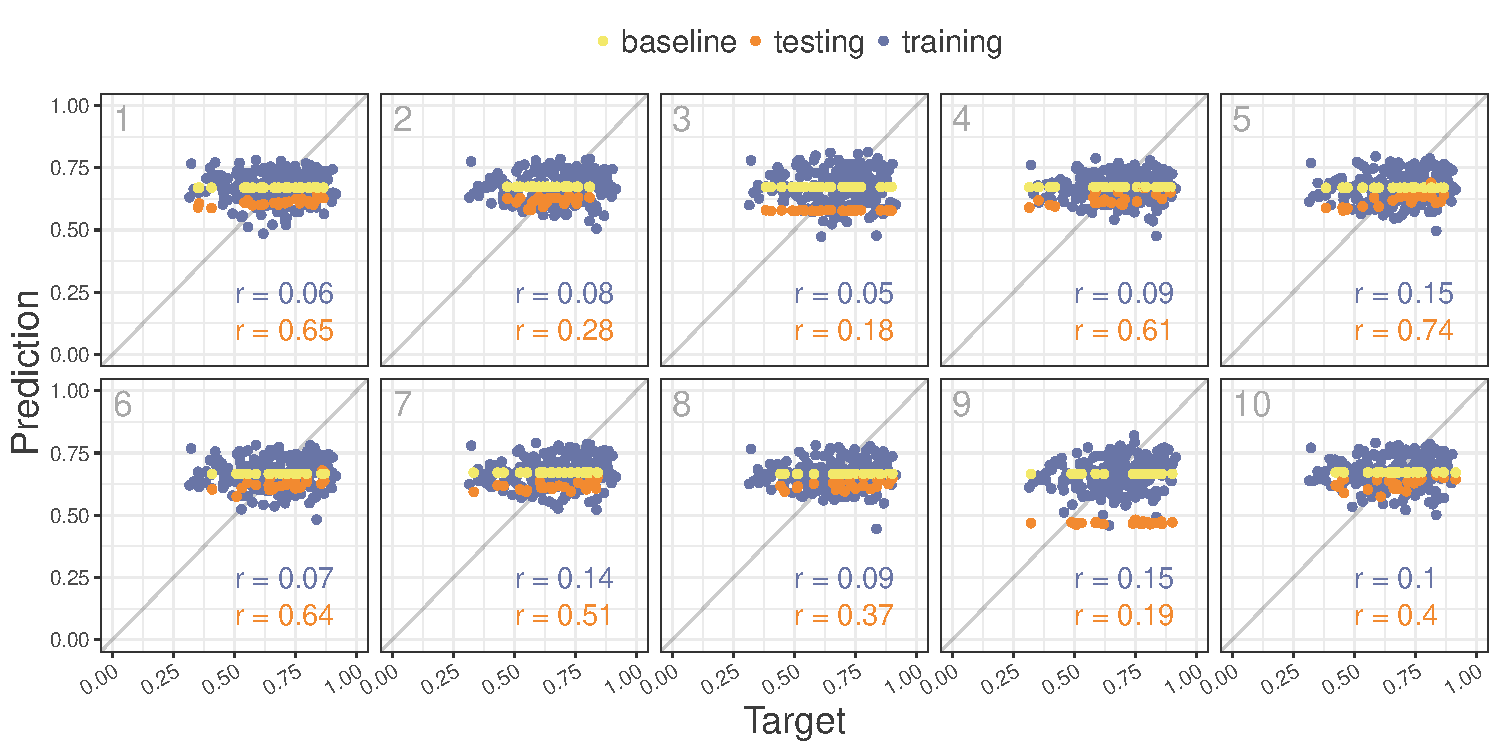
\includegraphics[width=\linewidth]{graphs/all-pred-target-epoch1.pdf}
	\caption{Testing label (x axis) vs. model prediction (y axis) before training; faceted over cross-validation configurations.}
	\label{fig:app-corr-pretraining}
\end{figure*}

\begin{figure*}[!htb]
	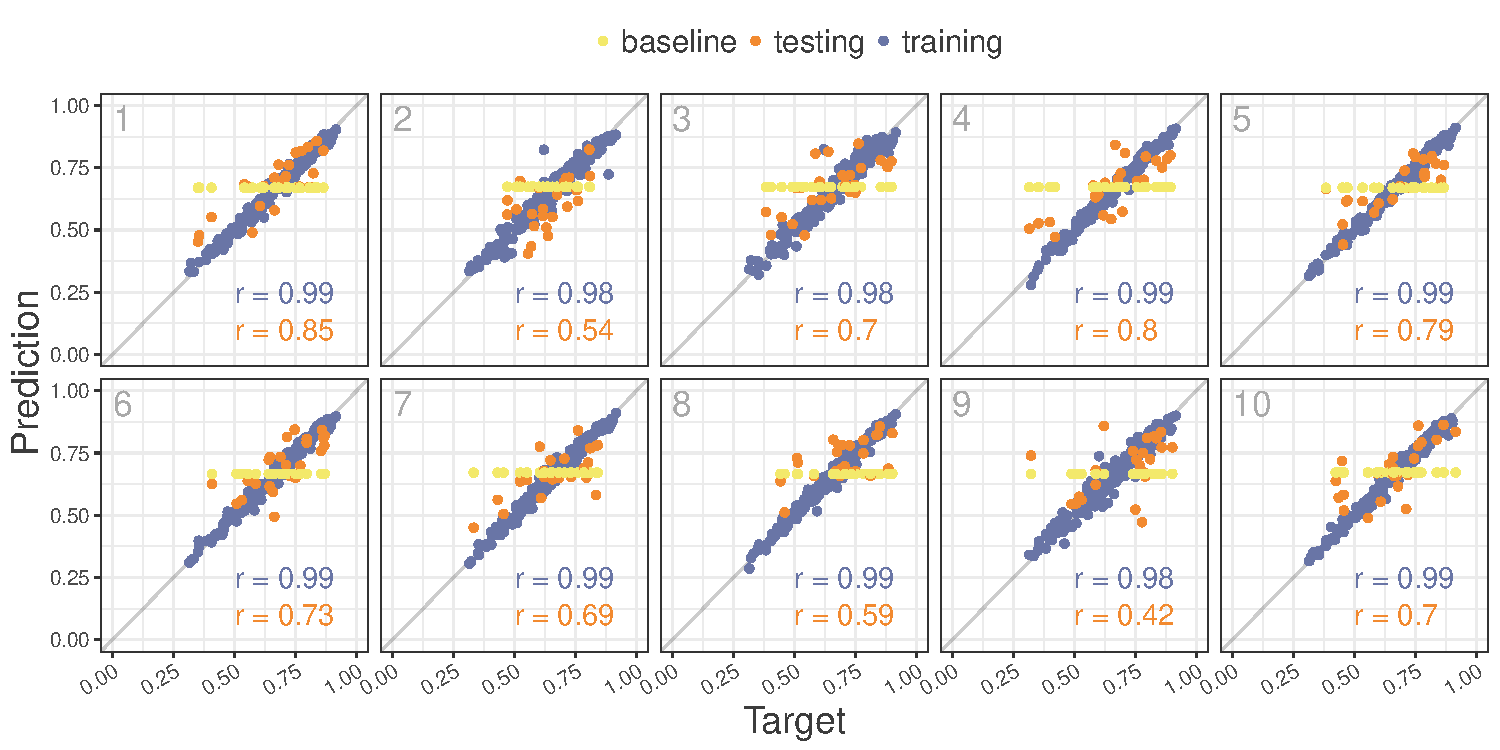
\includegraphics[width=\linewidth]{graphs/all-pred-target-epoch30.pdf}
	\caption{Testing label (x axis) vs. model prediction (y axis) after training; faceted over cross-validation configurations.}
	\label{fig:app-corr-posttraining}
\end{figure*}

\end{document}
